\documentclass{article}

\usepackage[spanish, boxed]{algorithm2e} %% Para algoritmos

% Símbolos
\usepackage{recycle}
\usepackage{amsfonts}

% Teoremas y pruebas
\usepackage{amsthm}

% Figuras
\usepackage{graphicx}

% Gráficas
\usepackage{tikz}

% Cambiando "Proof" por "Demostración"
\renewcommand*{\proofname}{Demostraci\'on}

% Cambiar "Figure" por "Figura"
\renewcommand{\figurename}{Figura}

%% Entrada y salida del algoritmo
\SetKwInput{KwInput}{Entrada}
\SetKwInput{KwOutput}{Salida}

% Estilo Tikz
\tikzstyle{edge}=[shorten <=2pt, shorten >=2pt,
                  >=stealth, line width=1.1pt]
\tikzstyle{vertex}=[circle, fill=white, draw,
                    minimum size=5pt,
                    inner sep=0pt, outer sep=0pt]

% Márgenes
\addtolength{\voffset}{-1cm}
\addtolength{\hoffset}{-1.5cm}
\addtolength{\textwidth}{3cm}
\addtolength{\textheight}{2cm}

% Encabezados y Pies de Página
\usepackage{fancyhdr}
% Información del Encabezado
\lhead{Teor\'ia de Gr\'aficas II 2021-2 \\
       Tarea 1}
\rhead{Profesor: C\'esar Hern\'andez Cruz \\
       Ayudante: Daniel Garc\'ia Argueta}
% Información del Pie de Página
\rfoot{\recycle}
\cfoot{\vspace{-0.8cm}?`Realmente necesitas imprimir esta hoja?}
\lfoot{\recycle}
\pagenumbering{gobble}
\footskip = 50pt
% Línea del encabezado
\renewcommand\headrulewidth{1.5pt}
%%%%%%%%%%%%%%%%%%%%%%%%%%%%%%%%%%%%%%%%%%%%%%%%%%%%%%%%%%%%%
%%%%%%%%%%%%%%%%%%%%%%%%%%%%%%%%%%%%%%%%%%%%%%%%%%%%%%%%%%%%%
%%%%%%%%%%          Gráfica en encabezado          %%%%%%%%%%
%%%%%%%%%%%%%%%%%%%%%%%%%%%%%%%%%%%%%%%%%%%%%%%%%%%%%%%%%%%%%
%%%%%%%%%%%%%%%%%%%%%%%%%%%%%%%%%%%%%%%%%%%%%%%%%%%%%%%%%%%%%
\makeatletter
\def\headrule{{\if@fancyplain\let\headrulewidth\plainheadrulewidth\fi
\hrule\@height\headrulewidth\@width\headwidth
\vspace{0.1cm}
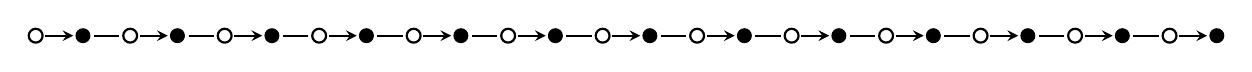
\begin{tikzpicture}
  \begin{scope}[scale=0.6]
   \foreach \x in {0,2,...,24} {
      \node [circle,draw,thick,inner sep=0,minimum size=5pt] (\x) at (\x,0){};
   }
   \foreach \x in {1,3,...,25} {
      \node [circle,draw,fill=black,inner sep=0,minimum size=5pt] (\x) at (\x,0){};
   }
   \foreach \x/\y in {0,2,...,24} {
     \pgfmathsetmacro\result{\x + 1}
     \draw [->,>=stealth,shorten <=3.5pt, shorten >=3.5pt,line width=0.7pt] (\x,0) to (\result,0);
   }
   \foreach \x/\y in {1,3,...,23} {
     \pgfmathsetmacro\result{\x + 1}
     \draw [>=stealth,shorten <=4pt, shorten >=4pt,line width=0.7pt] (\x,0) to (\result,0);
   }
   % \node [inner sep=0,minimum size=5pt] (25.5) at (25.5,-0.05){$\cdots$};
  \end{scope}
\end{tikzpicture}
\vskip-\headrulewidth
\vskip-1.5pt}}
\makeatother
%%%%%%%%%%%%%%%%%%%%%%%%%%%%%%%%%%%%%%%%%%%%%%%%%%%%%%%%%%%%%
%%%%%%%%%%%%%%%%%%%%%%%%%%%%%%%%%%%%%%%%%%%%%%%%%%%%%%%%%%%%%
%%%%%%%%%%%%%%%%%%%%%%%%%%%%%%%%%%%%%%%%%%%%%%%%%%%%%%%%%%%%%
%%%%%%%%%%%%%%%%%%%%%%%%%%%%%%%%%%%%%%%%%%%%%%%%%%%%%%%%%%%%%
%%%%%%%%%%%%%%%%%%%%%%%%%%%%%%%%%%%%%%%%%%%%%%%%%%%%%%%%%%%%%

% Estilo
\pagestyle{fancyplain}

% Macros
\newcommand{\set}[1]{\left\{ #1 \right\}}


\begin{document}

\begin{enumerate}
  \item Demuestre que si $D$ es una digr\'afica, entonces su
    condensaci\'on $D^\ast$ es ac\'iclica.

    \begin{proof}
      Sean $C_1, C_2, ..., C_n$ las componentes fuertemente
      conexas de $D$. Por definici\'on de condensaci\'on, $D^\ast$
      es la digr\'afica cuyos v\'ertices son exactamente
      $C_1, C_2, ..., C_n$ y cuyo conjunto de flechas cumple lo
      siguiente: existe una flecha de $C_i$ a $C_j$ si y solo si
      existe una flecha desde alg\'un v\'ertice de $C_i$ hacia
      alg\'un v\'ertice de $C_j$ en $D$.

      Ahora, procederemos por contradicci\'on. Supongamos que
      $D^\ast$ s\'i tiene un ciclo dirigido. Sin p\'erdida de
      generalidad, sea el ciclo $C = C_1, C_2, ..., C_k, C_1$.
      Podemos verlo en la figura~\ref{fig:cycle}.

      \begin{figure}[h]
        \centering
        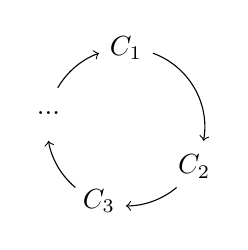
\begin{tikzpicture}[->]
          \node (i) at (90:1cm)  {$C_1$};
          \node (j) at (-30:1cm) {$C_2$};
          \node (k) at (250:1cm) {$C_3$};
          \node (l) at (170:1cm) {$...$};
          
          
          \draw (70:1cm)  arc (70:-10:1cm);
          \draw (-50:1cm) arc (-50:-90:1cm);
          \draw (230:1cm) arc (230:190:1cm);
          \draw (150:1cm) arc (150:110:1cm);
          
        \end{tikzpicture}
        \caption{Ciclo dirigido en $D^\ast$}
        \label{fig:cycle}
      \end{figure}

      Ahora, consideremos a $D'$, la subgráfica de $D$ inducida
      por el conjunto $\bigcup\limits_{i=1}^{k}C_i$. Veamos que
      $D'$ es fuertemente conexa. Para esto, consideremos
      a cualquier par de vértices $u$ y $v$ en
      $\bigcup\limits_{i=1}^{k}C_i$ y veamos que debe existir una
      trayectoria de $u$ a $v$ y otra trayectoria de $v$ a $u$.
      Primero, si ambos vértices pertenecen a la misma
      componente, entonces por definición de componente
      fuertemente conexa ya terminamos. Entonces supongamos que
      pertenecen a distintas componentes, digamos $C_u$ y $C_v$,
      respectivamente.

      Veamos que hay una trayectoria de $u$ a $v$. Es la que
      utiliza las siguientes flechas:

      \begin{itemize}
      \item Dentro de $C_u$, sigue la trayectoria desde $u$
        hasta el vértice que sale a la siguiente componente en el
        ciclo (dicha trayectoria existe porque $C_u$ es
        fuertemente conexa).
      \item De ahí, se va a la siguiente componente y al ser
        esta a su vez fuertemente conexa, puede también tomar una
        trayectoria que salga de ella y se dirija a la siguiente
        componente del ciclo.
      \item Hace esto hasta llegar a $C_v$.
      \item Una vez en $C_v$, tomamos la trayectoria hasta $v$,
        que existe por ser $C_v$ fuertemente conexa.
      \end{itemize}

      Por lo tanto, hay una trayectoria de $u$ a $v$. De manera
      análoga, hay una trayectoria de $v$ a $u$. Como $u$ y $v$
      eran vértices arbitrarios, entonces $D'$ es fuertememente
      conexa. Pero esto es una contradicción, ya que $D'$
      contiene a $C_1$, que es una componente fuertemenete
      conexa, lo que signficia que es maximal por contención.

      Por lo tanto, no puede haber un ciclo en $D^\ast$.
      
      
    \end{proof}
    
  \item Demuestre que si $D$ es una digr\'afica ac\'iclica, entonces
    tiene un \'unico n\'ucleo.   Adem\'as, a partir de su demostraci\'on
    obtenga un algoritmo para encontrar un n\'ucleo en una digr\'afica
    ac\'iclica.   ?`Qu\'e complejidad tiene su algoritmo?
    
    \begin{proof}
      
      Tenemos que hacer tres observaciones.
      
      \begin{enumerate}
      \item \label{itm:kernel} Si la digr\'afica tiene sumideros, entonces estos
        deben estar en el n\'ucleo. Esto es debido a que el n\'ucleo es un
        conjunto absorbente y nadie absorbe a un sumidero.
        
      \item \label{itm:neighbors} Los vecinos de los sumideros \textbf{no} pueden estar en el
        n\'ucleo. Esto debido a que el n\'ucleo es independiente y los sumideros
        est\'an en \'el.      
        
      \item \label{itm:sumi} Toda digr\'afica ac\'iclica tiene al menos
        un sumidero. Para ver esto, supongamos que no es as\'i y sea $T = v_1, v_2,
        v_3, ..., v_m$ la trayectoria dirigida de mayor longitud. Como no hay
        sumideros, en particular $v_m$ no es un sumidero. Entonces $v_m$ debe
        tener un exvecino. El exvecino no puede estar en la trayectoria, pues
        tendr\'iamos un ciclo dirigido. Entonces el exvecino es $v_{m+1}$, un
        v\'ertice fuera de la trayectoria. Pero entonces tenemos una trayectoria
        m\'as larga $v_1, v_2, ..., v_{m+1}$, contradiciendo la hip\'otesis de que
        $T$ era la trayectoria m\'as larga.
      \end{enumerate}
      
      
      Con estas observaciones, podemos proceder a hacer una prueba por
      inducci\'on sobre el n\'umero de v\'ertices de la gr\'afica. 
      
      \begin{itemize}
      \item \textbf{Base de inducci\'on:}
        Sea $D$ una digr\'afica con un solo v\'ertice $v$. Clarmente $\{v\}$ es el
        \'unico n\'ucleo de $D$.
      \item \textbf{Hip\'otesis de inducci\'on:}
        Supongamos que la propiedad se cumple para todas las digr\'aficas ac\'iclicas de
        orden menor o igual que $k$ para alguna $k$ en los naturales.
      \item \textbf{Paso inductivo:}
        Demostraremos la propiedad para las digr\'aficas de orden $k+1$.
        
        Sea $D$ una digr\'afica de \'orden $k+1$ y sea $S$ el conjunto de sus
        sumideros. Por la observaci\'on~\ref{itm:sumi} $S$ es no
        vac\'io.
        
        Sea $C = S \cup N(S)$. Tenemos dos casos. Si $C = V(D)$, entonces por
        las observaciones~\ref{itm:neighbors} y~\ref{itm:kernel}, el n\'ucleo debe
        contener a $S$ y no contener a $N(S)$. Como estos son todos los v\'ertices
        de la digr\'afica, el n\'ucleo es el conjunto $S$ y terminamos.

        Si, en otro caso $C \subset V(D)$, entonces nos fijamos en la digr\'afica
        $D' = D \setminus C$. Como $S$ era no vac\'io, esta digr\'afica tiene orden
        $k$ o menor y podemos aplicarle la hip\'otesis de inducci\'on, por lo que
        tiene un \'unico n\'ucleo $K'$. Observemos que $K = K' \cup S$ es un n\'ucleo para
        $D$, ya que:

        \begin{itemize}
          \item Es independiente. Para ver esto, consideremos a dos v\'ertices
            $v_1$, $v_2$ en $K$. Tenemos tres casos:
            \begin{enumerate}
              \item Si $v_1$ y $v_2$ est\'an ambos en $K'$, son independientes por
                ser parte de un n\'ucleo.
              \item Si ambos est\'an en $S$, son independientes por ser ambos
                sumideros de $D$.
              \item Si hay uno en $K'$ y otro en $S$, son independientes pues
                $K' \cup N(S) = \emptyset$ por construcci\'on.
              \end{enumerate}
            \item Es absorbente, ya que todo v\'ertices en $D' \setminus K'$ es absorbido por
              $K'$ y todo v\'ertice en $N(S)$ es absorbido por $S$.
            \end{itemize}
            Por lo tanto $K$ es n\'ucleo de $D$. Ahora, veamos que es
            \'unico. Supongamos que existe otro n\'ucleo $Q$. Fij\'emonos en $Q' = Q
            \setminus (S \cup N(S))$. $Q'$ debe ser un n\'ucleo para $D'$, ya que
            ning\'un v\'ertice en $D'$ es absorbido por $S \cup N(S)$. Pero como
            $K'$ era \'unico por hip\'otesis de inducci\'on, entonces $Q' = K'$ y por
            lo tanto $Q = K$.
      \end{itemize}
    \end{proof}

    A partir de esta demostraci\'on, obtenemos el algoritmo~\ref{alg:nucleo} para obtener
    el n\'ucleo de una digr\'afica ac\'iclica.
    
    \begin{center}
      \begin{algorithm}[H]
        \SetAlgoLined
        \KwInput{$D$ digr\'afica}
        \KwOutput{$K$ el n\'ucleo de D}
        $K \gets \emptyset$\;
        \While{$V(D) \neq \emptyset$}{
          $S \gets$ sumideros en D\;
          $K \gets K \cup S$\;
          $D \gets D \setminus (S \cup N(S))$\;
        }
        \KwRet{$K$}
        \caption{Algoritmo para obtener el núcleo de una digráfica acíclica}
        \label{alg:nucleo}
      \end{algorithm}

      El algoritmo tiene complejidad $O(|V|³ + |V|²|E|)$. El ciclo \texttt{while} se repite
      a lo m\'as tantas veces como v\'ertices, pues se quita un conjunto no
      vac\'io de v\'ertices a $D$ en cada iteraci\'on. Obtener $S$ toma tiempo
      lineal, pues es recorrer los v\'ertices y ver cu\'ales tienen exgrado
      $0$. Unir $K$ y $S$ tambi\'en toma tiempo lineal. Quitar un v\'ertice es
      $O(|V| + |E|)$ y se hace potencialmente $|V|$ veces. Por lo tanto, quitar
      $S$ tiene complejidad $O(|V|² + |V||E|)$ y al multiplicar por $O(|V|)$ del
      ciclo, obtenemos la complejidad previamente mencionada.
    \end{center}

  \item Demuestre que cualquier digr\'afica con al menos dos n\'ucleos
    contiene un ciclo par.

    \begin{proof}
      Sea $D$ una digráfica con al menos dos núcleos $K_1$ y $K_2$.
    \end{proof}
    
  \end{enumerate}
\end{document}
